% legible-motion-bench: HRI 2027 Short Contribution, code track.
%
% ACM sigconf, the format the call requires. The class is
% vendored: acmart.cls is generated from acmart.ins by the Makefile, so
% the build does not depend on the local TeX distribution shipping it.
%
% Two builds, one source. `make` produces the anonymised submission
% build, which HRI requires: [sigconf,anonymous,review], line numbers on,
% and the mandatory ACM reference format left in place. `make named`
% defines NAMEDBUILD and produces paper-named.pdf with the author block
% and no rights block, which is the preprint.
%
% Nobody edits a line to switch. Doing that by hand is how a submission
% goes out with the wrong class, and it happened here often enough to be
% worth removing as a possibility.
%
% Four pages excluding references. The track is judged on accessibility,
% completeness, utility and relevance, which is why Availability and use
% is a section rather than a closing line. Every number below comes from
% paper/generated/, written by tools/build_paper_results.py from the
% committed records. None of them is typed by hand. See paper/STATUS.md
% for the honest state of each section.

\ifdefined\NAMEDBUILD
  \documentclass[sigconf,nonacm]{acmart}
  \settopmatter{printacmref=false}
  \renewcommand\footnotetextcopyrightpermission[1]{}
\else
  \documentclass[sigconf,anonymous,review]{acmart}
\fi

\usepackage{booktabs}

% Without this both builds print acmart's placeholder, Conference'17,
% July 2017, Washington, DC, USA, in the running head. Rights, ISBN and
% DOI are deliberately not set: those are camera-ready values and
% inventing one is worse than leaving the placeholder.
\acmConference[HRI '27]{Proceedings of the 2027 ACM/IEEE International
  Conference on Human-Robot Interaction}{March 8--12, 2027}{Santa Clara,
  CA, USA}
\acmYear{2027}
\copyrightyear{2027}

\begin{document}

\title{What Clarity Costs: Measuring Legible Robot Motion Against Path
Cost and Constraint Satisfaction}

\author{Munawar Kazmi}
\affiliation{%
  \institution{Independent}
  \city{Multan}
  \country{Pakistan}
}
\email{munawarsaeedkazmi1@gmail.com}

\begin{abstract}
A robot heading for one of several goals is unreadable for the first
seconds of its motion, when a person nearby hesitates or steps into its
path. Legible motion deviates early to resolve that, the deviation costs
path length, and it can also cost the constraint the robot was meant to
respect. We contribute a judge-free benchmark measuring all three:
legibility in Dragan et al.'s form, path cost against the exact optimum,
and satisfaction of stated keep-out zones. Eight worlds carry 46
machine-checked geometric facts, cost-to-go is the exact geodesic over a
visibility graph, and no human rater or model judge appears in the
scoring loop. Every table is recomputed from committed records, and
anything emitting a trajectory can be scored. Three language models
produced 480 trajectories under four stated path budgets. Two claimed
legibility for all 320 of theirs, 93 of which were not physically
possible, and paid the same whatever they were told. The third stayed
feasible on all 160 and moved with the budget at every step.
\end{abstract}

% Mandatory for papers over two pages, which this became when related
% work was added.
%
% Generated by ACM's own tool at dl.acm.org/ccs on 4 September 2026 and
% pasted whole, which is the only way this block is allowed to be
% written. It was incomplete until then: Motion path planning was
% declared with \ccsdesc and left out of the XML, because its identifier
% could not be sourced and a guess at it turned out to be Multi-agent
% systems. The tool gives it as 10010147.10010178.10010213.10010215,
% Computing methodologies, Artificial intelligence, Control methods,
% Motion path planning. The two identifiers that had been sourced by
% hand came back from the tool unchanged, which is what says the sourcing
% was sound and not that it happened to agree.
\begin{CCSXML}
<ccs2012>
   <concept>
       <concept_id>10010520.10010553.10010554</concept_id>
       <concept_desc>Computer systems organization~Robotics</concept_desc>
       <concept_significance>500</concept_significance>
       </concept>
   <concept>
       <concept_id>10003120.10003121</concept_id>
       <concept_desc>Human-centered computing~Human computer interaction (HCI)</concept_desc>
       <concept_significance>300</concept_significance>
       </concept>
   <concept>
       <concept_id>10010147.10010178.10010213.10010215</concept_id>
       <concept_desc>Computing methodologies~Motion path planning</concept_desc>
       <concept_significance>300</concept_significance>
       </concept>
 </ccs2012>
\end{CCSXML}

% The XML above is the tool's output pasted whole. The order of the
% three lines below is not: it is the order the build had before the
% identifier was sourced, restored because the tool's order breaks the
% printed CCS Concepts line badly enough to overrun the column by
% 12.41pt. These lines set what is printed and carry no identifiers, so
% ordering them is a typesetting choice and not a change to the
% classification.
\ccsdesc[500]{Computer systems organization~Robotics}
\ccsdesc[300]{Computing methodologies~Motion path planning}
\ccsdesc[300]{Human-centered computing~Human computer interaction (HCI)}

\keywords{legibility, human-robot interaction, motion planning,
benchmarking, language models}

\maketitle

\section{Introduction}

Legibility is not ours. Dragan et al.~\cite{dragan2013legibility}
formalised it: a legible trajectory is one that departs from the
efficient path early enough for an observer to infer the goal sooner
than efficiency alone would allow. What is missing from that literature
is a price. Deviating for clarity moves the robot somewhere it would not
otherwise go, and in a real room that somewhere is occupied.

The literature notices this and leaves it qualitative: what a legible
trajectory costs in satisfaction of a stated constraint is not an axis of
any reported result.

This report contributes an instrument rather than a planner: a
reproducible way to ask what a given trajectory pays, in path and in
constraint satisfaction, for the clarity it buys.

What is released is the instrument, not a result that happens to have
code attached. It is eight worlds, each carrying the facts about its own
geometry that a test re-checks against the implementation; an observer
and three metrics with no free parameter in the ones the headline rests
on; an exact optimal cost-to-go to measure path cost against; a
legibility optimiser and a shortest-path baseline to compare a candidate
trajectory with; the prompt template, carried by SHA-256 into every
record so a comparison is of models and not of prompts; and the tools
that turn committed records into the tables and the figure printed here.
The worlds and the facts they carry are the fixed part. What is measured
against them is not: anything that emits a sequence of positions can be
scored, and the cost of adding a planner or a model is one record file.
Scoring is a separate step from asking, so a metric can be recomputed
from replies already given without spending an API call.

We use it here to ask whether language models produce legible motion when
told to, which is a demonstration of the instrument rather than the
reason it exists.

\section{Related work}

Legibility in the sense used here is Dragan et al.'s: an observer with a
Boltzmann-rational model of the robot infers the goal from motion, and a
legible trajectory is one that raises that inference early
\cite{dragan2013legibility}. Both founding papers bound what the robot may
spend on it. The HRI paper subtracts a cost regulariser from the objective
and the RSS paper constrains the trajectory to a trust region, in both
cases because a robot can otherwise make a trajectory ever more legible at
ever greater cost \cite{dragan2013generating}. The ceiling we sweep is the
hard variant of that bound, expressed as a ratio against the optimal path
rather than as an absolute in a cost functional.

What legibility does to the space around the robot is stated in that
literature before it is measured. The RSS paper reports that legibility
moves the trajectory much closer to an obstacle in order to disambiguate
between two goals, and leaves it there: obstacles enter as a soft penalty
inside the objective, clearance is never reported as a number, and
constraint satisfaction is not an axis of any result
\cite{dragan2013generating}. Legibot likewise carries obstacle distance
and rate of approach as terms in a task cost, reports legibility scores
from a user study, and gives no quantitative comparison of path cost
against the baseline \cite{amirian2024legibot}. Closest to this report is
legible navigation among moving agents, which does put a safety quantity
beside legibility in one table, reporting minimum separation and minimum
time to collision \cite{bastarache2023legible}. What differs here is which
quantity and in what form: satisfaction of a stated static constraint
rather than proximity to moving agents, traced as a curve against a path
budget rather than compared between policies.

On evaluation, the guidelines for social robot navigation call for
repeatable benchmarking criteria, endorse algorithmic metrics as cheap to
compute and reproducible, name legibility as a principle, and point at
Dragan for its definition rather than stating a computed metric of their
own \cite{francis2025principles}. They also set the condition this
instrument does not meet, that objective metrics be validated empirically,
which the limitations take up. The alternative is to evaluate legibility
frameworks against human observers on framework-independent trajectories
\cite{wallkotter2022evaluating}. That is the harder experiment and it
measures something this one does not: an exactly computed observer is
reproducible rather than right.

Language models have been asked for expressive robot behaviour before.
GenEM prompts GPT-4 to reason about social context and emit control code
for a mobile robot, producing behaviours such as nodding or excusing
itself through speech, body movement and a light strip
\cite{mahadevan2024generative}. The pairing is the same and the quantity
is not. Legibility in Dragan's sense does not appear in that work, no
observer infers a destination anywhere in it, and the behaviours are
judged by participants watching video clips on seven-point scales against
a professional animator's versions. What is asked for here is narrower and
checkable: a trajectory under a stated path budget, in a world whose
optimal cost-to-go is computed exactly.

\section{The instrument}

Everything is 2D and kinematic. A trajectory is a sequence of positions
traversed at constant speed. There is no physics engine, which is a
scope decision: physics would improve the pictures and change none of
the numbers.

The observer is Boltzmann-rational in exactly the form of
\cite{dragan2013legibility}, equation~8, and our legibility metric is
their equation~9 including the weighting $f(t) = T - t$. Both were
compared line by line against the implementation. Our only addition is an
inverse temperature, which is recorded in the observer's name in every
result.

Two observers are implemented and every number here uses the first. One
takes cost-to-go to be the obstacle-aware geodesic; the other takes it to
be the straight line, modelling someone who can see the robot and knows
the candidate goals but not what stands between them. That is a
measurement decision rather than an ablation, and it changes the
measurement. Along the cheapest route in the world with a wall to round,
the informed observer holds at the prior of exactly 0.5000 and learns
nothing, while the naive one falls to 0.3164, because from a viewpoint
that cannot see the wall the robot is walking away from the goal it is
going to. Legibility on that one path is 0.5457 read the first way and
0.4370 read the second.

That posterior rests on the optimal cost-to-go, so we compute it exactly
rather than approximately. Obstacles are convex polygons, the shortest
obstacle-avoiding path is a polyline through their vertices, and the
optimum comes from search over the visibility graph: no grid, no
resolution to defend. The geometric predicate underneath is guarded, decided
in floating point wherever an error bound proves the sign cannot have
changed and in exact rational arithmetic otherwise. On 20{,}000
near-collinear cases an unguarded floating point determinant returns the
wrong sign on more than a tenth of them; the guarded predicate matches
rational arithmetic on all of them, and the test suite asserts both
halves so the corpus cannot quietly become easy.

Keep-out zones do not block motion. A trajectory may cross one and is
scored for having done so. If they blocked motion there would be no
trade to measure.

The code is tested rather than merely posted. A suite of 248 tests runs
in continuous integration and re-checks all 46 facts the worlds carry
against the committed implementation, so a change that alters a world's
geometry fails the build instead of quietly moving a published number.
Tests assert on trajectory arrays and metric values and never on rendered
image bytes, and a figure is treated as a drawing of numbers that have
already been verified elsewhere.

Legibility optimisation is bounded by a ceiling on the cost ratio. That
bound is not our idea: \cite{dragan2013legibility} adds a cost
regulariser and \cite{dragan2013generating} a hard trust region, both
because a robot can otherwise make a trajectory ever more legible at ever
greater cost. Sweeping the ceiling turns a single trajectory into a
frontier.

\section{What language models do}

The prompt states the room, the goals, which goal the robot is going to,
the obstacles, the keep-out zones, and a path budget in absolute units.
It asks for a trajectory that makes the destination clear as early as
possible, and asks the model to judge its own answer. Temperature 0.7,
five samples per world, eight worlds.

% Both results tables are wider than one column at three models. They
% span the page rather than being shrunk below what a reviewer can read.
\begin{table*}[t]
\centering
\small
% Generated by tools/build_paper_results.py from results/*.jsonl and
% configs/model_manifest.json. Do not edit by hand; rerun the tool
% after any completed run.

\begin{tabular}{lrr}
\toprule
Over 40 decodes each & Llama 3.3 70B & Qwen 2.5 7B \\
\midrule
replies that parsed & 40 & 40 \\
called legible by the model & 40 & 40 \\
physically possible & 29 & 26 \\
clearer than the shortest path & 20 & 10 \\
over the stated path budget & 15 & 9 \\
entered a keep-out zone & 7 & 7 \\
\bottomrule
\end{tabular}

\caption{Counts at a stated path budget of 25 per cent. Of 120 decodes,
116 claimed to be legible, including the 25 that were not physically
possible. All four refusals came from one model, and none of them
survives raising the stated budget to 2.00.}
\label{tab:models}
\end{table*}

% Declared here rather than beside the text that discusses it. A double
% column float cannot be set on the page that is current when it is
% declared, so at its point of discussion it was deferred past the start
% of the references and printed on a page of its own after them.
\begin{table*}[t]
\centering
\small
% Generated by tools/build_paper_results.py from results/*.jsonl and
% configs/model_manifest.json. Do not edit by hand; rerun the tool
% after any completed run.

\begin{tabular}{rrrrr}
\toprule
& \multicolumn{2}{c}{Llama 3.3 70B} & \multicolumn{2}{c}{Qwen 2.5 7B} \\
Stated budget & median cost & over & median cost & over \\
\midrule
1.10 & 1.2817 & 30 & 1.1663 & 17 \\
1.25 & 1.2817 & 15 & 1.1588 & 9 \\
1.50 & 1.2817 & 10 & 1.1712 & 3 \\
2.00 & 1.2817 & 0 & 1.1709 & 0 \\
\bottomrule
\end{tabular}

\caption{Forty decodes at each stated budget, per model. All three are
swept across all four budgets, 480 decodes in the grid. The budget nearly
doubles across it. Two of the three pay the same either way; the third
pays more at every step.}
\label{tab:ceilings}
\end{table*}

\begin{figure}[t]
\centering
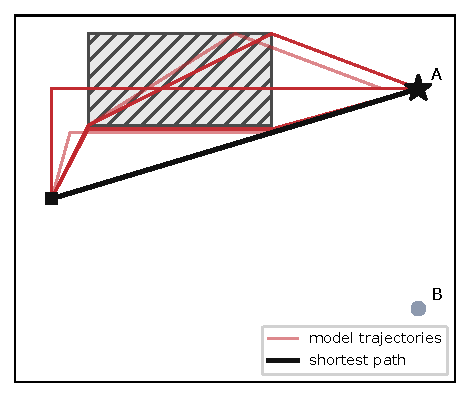
\includegraphics[width=\columnwidth]{generated/keep_out_shortcut}
\caption{The world built so that the clearest signal is the one the robot
may not send. The cheapest route to the true goal A (black) stays clear
of the keep-out zone (hatched), so safety costs nothing until a planner
tries to be legible. All fifteen trajectories the three models returned
(red, five samples each) are more legible than the shortest path. Ten of
them cross the zone and five do not, and the five that stay out are one
model's, on five of five samples. Drawn from the committed records, not
by hand.}
\Description{Plan view of an empty room twelve units wide and ten deep.
The robot starts at the middle of the left edge. On the right are two
goals: the true goal A, marked with a star, above, and goal B, marked
with a small circle, below. A hatched rectangle across the upper left of
the room is the keep-out zone. A thick black line, the shortest path,
runs straight from the start to A and passes just under the hatched
rectangle without touching it. Fifteen thin red lines, the model
trajectories, leave the start on a higher course and come down to A. Ten
of them pass through the hatched rectangle and five bend just under its
lower edge without entering it.}
\label{fig:keepout}
\end{figure}

What the three models share is thin, and what separates them is not.

They agree in one world. Where the true goal lies between the other two,
all fifteen decodes were physically possible and none beat the shortest
path, which is what \cite{dragan2013legibility} predicts when
exaggeration towards a middle goal points at a different goal.

Elsewhere the differences are the result. In the world with a wall to
round, one model returned a physically impossible trajectory on all five
samples, one on one of five, and one on none. In the world built so that
the clearest signal and the keep-out zone conflict
(Figure~\ref{fig:keepout}), all three beat the shortest path on five of
five. Two of them entered the zone on five of five; the third entered on
none, threading a route under the boundary at a cost ratio between 1.0819
and 1.1057. The constraint was satisfiable with the clarity still
available, and the first two give no sign of having looked for that.

The claim behaves the same way, and changing the budget shows what it is
worth. Two models called every one of their 80 trajectories legible,
including 25 that were not physically possible. The third declined four
times at a stated budget of 1.25, three in the middle-goal world and one
in the world with the wall, which reads like a model that knows when
deviating cannot help. It is not that. In the middle-goal world it
returns the identical trajectory under both budgets, the straight line
through $(1,5)$ and $(11,5)$, scoring exactly the baseline. That
trajectory is called not legible on three of five samples at 1.25 and
legible on five of five at 2.0. Same world, same motion; only the number
in the prompt changed.


Table~\ref{tab:ceilings} asks whether the budget violations mean the
budget was too tight or that the budget was not attended to. For two of
the three models it is the second. One model's median cost moves by
0.0124 across a budget that nearly doubles and the other's does not move
at all, staying at 1.2817 to four places in all four rows, so their
falling violation counts are the line moving and not the models
complying. Where the optimiser sits exactly on the budget in every row,
because for a planner it is a constraint, for those two it is text.

The third model separates the two readings that compliance at a single
budget cannot. Its pooled median rises at every step of the grid, 1.0536
at a stated 1.10, then 1.0819, 1.1116 and 1.1539, so this is a response
to the budget rather than two points that happen to differ. Given 2.0
rather than 1.25 it spends more in seven of the eight worlds. Where
the extra room buys something it takes much more of it: in the keep-out
world the median cost goes from 1.0819 to 1.4139 and legibility with it,
0.7710 to 0.8496, without a single keep-out entry at any of the four. In
the world with a wall to round it crosses from below the shortest path's
legibility to well above it, 0.5339 to 0.7575 against a baseline of
0.5457. In the world where the true goal lies between the others it
returns the same straight line under both budgets and spends nothing
extra. It never exceeded any of the four stated budgets.

\section{Limitations}

Validity is the limitation that matters, so it goes first. The metric
here is not a new claim about people. It is equation~9 of
\cite{dragan2013legibility} computed exactly rather than approximately,
so whatever validity it has is inherited from that paper's user studies,
and it is bounded where those authors bounded it, inside the trust
region. That is why nothing outside a stated cost ceiling is reported
here. What this instrument adds is reproducibility, not correspondence.
Judge-free is not judge-proof.

Two statements have to be kept apart, and only the first is supported by
anything here: that a trajectory scores higher under the stated observer
model, and that a person would read it sooner. Nobody has watched these
trajectories. The guidelines for social navigation put the same order on
it, recommending algorithmic metrics first and asking that objective
metrics later be validated empirically~\cite{francis2025principles}; this
report is at the first step and not the second. What would settle it is a
study in which people see these trajectories and say which goal they
believe, set against the posterior that scored them. Every trajectory is
committed, one JSON object per line, so that study needs participants
rather than a reimplementation. Comparing legibility frameworks against
human observers remains the harder and more informative
experiment~\cite{wallkotter2022evaluating}.

Three narrower limits. With more than one goal the legibility score
cannot reach 1, so a value of 0.93 is not 93 per cent of anything. Our
observer has no option for a goal outside the declared set, though real
observers form exactly that belief when motion becomes strange enough.
And time to confidence, the one metric here with a free parameter, is not
stable: across the admissible band the count of trajectories reaching
confidence sooner than the baseline runs from 234 of 387 down to 144 of
387 across the whole grid, and individual verdicts move with it: 72 of
the 387 differ between the default and the loosest threshold. It is reported nowhere above and no
claim here rests on it.

Three models at one temperature over eight worlds is a pilot. Every number
here is recomputed by a committed tool from committed records.

\section{Availability and use}

The eight worlds and the facts each one carries, the prompt template,
every record file behind the tables above, and the tools that recompute
every table and the figure from those records, are public under the MIT
licence. The link is withheld here for anonymous review and an anonymised
copy accompanies this submission; the link is given at camera-ready.
Nothing reported above was produced by a step that is not in that
repository.

It runs on Python 3.10 with no third-party package. \texttt{pytest} runs
the 248 tests; one further command re-checks the 46 facts the worlds
carry against the code, and another prints the suite inventory that every
denominator in this report comes from. Matplotlib is needed only to draw
figures and nothing else imports it. The tables and the figure above are
written from the record files by two committed tools, so a reader who
doubts a number can regenerate it rather than take it.

Adding a planner is one class with a \texttt{plan} method that takes a
world and returns a sequence of positions. Adding a model is one backend
with a \texttt{complete} method that takes a prompt and returns the
reply as a string. Both are then scored by the code that scored
everything here, because scoring takes a trajectory and a world and knows
nothing about what produced either. Scoring is deliberately not done
inside the runner: records hold the replies and a separate tool holds the
arithmetic, so changing a metric cannot rewrite what a model said. Worlds
are JSON, validated strictly in both directions, an unknown key being an
error, because a misspelled \texttt{keep\_out\_zones} would otherwise
load as a world in which every planner scores as perfectly safe.

So the instrument is not specific to language models. Anything that emits
a trajectory can be scored by it, and the cost of adding a planner or a
model is one record file. The worlds and the facts they carry are the
fixed part; what gets measured against them is not.

\section{Responsible use}

No human participants and no personal data are involved at any point.
Replies are committed as they came back. The 292 failed requests are
recorded as evidence and retried rather than dropped, and the paths that
turned out to be impossible are kept and counted rather than filtered
out, since a record set holding only what worked would misstate the
models it names.

Two readings of these numbers should be refused in advance. A legibility
score is not a safety certificate: a keep-out zone stands in for a stated
spatial constraint, and a trajectory that respects one has satisfied a
declared rule rather than been shown to be safe near a person. That is
the same boundary the limitations draw around the metric itself. And a
model's standing here is its standing on this instrument, under one
prompt at one temperature, rather than a general claim about the model;
the exact checkpoint that answered is recorded in every record so a later
run can be compared rather than assumed comparable.

\bibliographystyle{ACM-Reference-Format}
\bibliography{references}

\end{document}
